\documentclass[../main.tex]{subfiles}

\begin{document}
 \section{Crittografia Asimmetrica}
\label{sec:crittografia-asimmetrica}

\subsection{Schema e Concetti Fondamentali}
La crittografia asimmetrica, o a chiave pubblica, si basa sull'uso di una coppia di chiavi (keypair) per ogni partecipante.
\begin{itemize}
    \item \textbf{Chiave Pubblica ($k_1$ o $K_{pub}$):} Può essere distribuita liberamente, anche su canali insicuri. Viene usata per cifrare i messaggi destinati al proprietario della coppia di chiavi.
    \item \textbf{Chiave Privata ($k_2$ o $K_{priv}$):} Deve essere mantenuta segreta dal suo proprietario. Viene usata per decifrare i messaggi ricevuti.
\end{itemize}

Lo schema generico per la \textbf{confidenzialità} è il seguente:
\begin{enumerate}
    \item Bob vuole inviare un messaggio $m$ ad Alice.
    \item Bob ottiene la chiave pubblica di Alice, $K_{pubA}$ (es. tramite un canale insicuro).
    \item Bob cifra il messaggio usando la chiave pubblica di Alice: $c = E_{K_{pubA}}(m)$.
    \item Alice riceve il messaggio cifrato $c$.
    \item Alice usa la sua chiave privata, $K_{privA}$, per decifrare il messaggio: $m = D_{K_{privA}}(c)$.
\end{enumerate}

\begin{figure}[H]
  \centering
  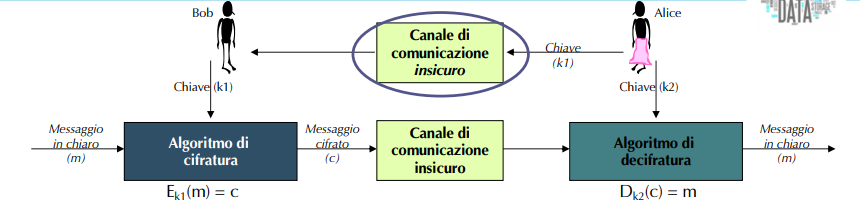
\includegraphics[width=0.8\textwidth]{asymm-gen.png}
  \caption{Schema generico crittografia asimmetrica}
  \label{fig:}
\end{figure}

La proprietà fondamentale è che, data la chiave pubblica $k_1$, deve essere computazionalmente impossibile (molto difficile) ricavare la corrispondente chiave privata $k_2$.
Mentre questo risolve il problema della distribuzione sicura della chiave di cifratura, introduce un nuovo problema: garantire l'\textbf{autenticità} della chiave pubblica $k_1$.

\subsection{Obiettivi e Basi Teoriche}
I meccanismi asimmetrici servono a tre scopi principali:
\begin{enumerate}
    \item \textbf{Confidenzialità:} Proteggere il contenuto del messaggio (come visto sopra).
    \item \textbf{Firme Digitali:} Fornire autenticazione del mittente, integrità del messaggio e non ripudio.
    \item \textbf{Instaurazione di Chiavi Effimere:} Scambiare in modo sicuro una chiave di sessione (es. simmetrica), come fa il protocollo Diffie-Hellman.
\end{enumerate}

Questi meccanismi basano la loro sicurezza sulla difficoltà (ad oggi) nel risolvere alcuni problemi della teoria dei numeri. Si usano operazioni "unidirezionali":
\begin{itemize}
    \item \textbf{Semplici da calcolare:} Es. $n = p \cdot q$ (moltiplicazione di due primi).
    \item \textbf;Difficili da invertire:} Es. trovare $p$ e $q$ dato $n$ (fattorizzazione di interi).
\end{itemize}
La sicurezza non è provata in assoluto, ma si basa sul fatto che i problemi matematici sottostanti sono studiati da secoli e ancora non si conoscono algoritmi efficienti per risolverli (es. in tempo polinomiale).

\subsection{Richiami: Teorema di Eulero}
L'algoritmo RSA si basa su concetti di aritmetica modulare, in particolare sul Teorema di Eulero.
\begin{itemize}
    \item Si definisce $Z_n$ come l'insieme dei numeri modulo $n$ (i resti della divisione per $n$).
    \item Si definisce $Z_n^*$ come il sottoinsieme di $Z_n$ che contiene i numeri primi relativi a $n$ (cioè $mcd(x,n)=1$).
    \item La \textbf{Funzione $\phi(n)$ di Eulero} conta quanti numeri ci sono in $Z_n^*$ (la sua cardinalità: $\phi(n) = |Z_n^*|$).
    \item Se $n$ è un numero primo, $\phi(n) = n-1$.
    \item Se $n = p \cdot q$, con $p$ e $q$ primi distinti, allora $\phi(n) = (p-1)(q-1)$.
    \item \textbf{Corollario del Teorema di Eulero (base di RSA):} Dati $p, q$ primi, $n=pq$, per ogni $m \in Z_n$ e $k \ge 0$ vale:
    $$ m^{k \cdot \phi(n) + 1} = m \mod n $$
\end{itemize}
Questo corollario ci dice che se troviamo due numeri $e$ e $d$ tali che $e \cdot d = 1 \mod \phi(n)$ (cioè $e \cdot d = k \cdot \phi(n) + 1$ per qualche $k$), allora l'operazione di "elevamento a $e$" è l'inversa dell'operazione di "elevamento a $d$".
Infatti: $(m^e)^d \mod n = m^{ed} \mod n = m^{k \cdot \phi(n) + 1} \mod n = m \mod n$.

\section{Algoritmo RSA (Rivest, Shamir, Adleman)}
RSA (1977) è il primo e più noto meccanismo asimmetrico "tuttofare", utilizzabile per tutti e tre gli obiettivi (confidenzialità, firme, scambio chiavi). Basa la sua sicurezza sulla difficoltà di fattorizzare $n$.

\subsection{Generazione delle Chiavi}
I parametri di RSA sono:
\begin{enumerate}
    \item \textbf{Parametri Privati (segreti):}
          \begin{itemize}
              \item Si scelgono due numeri primi $p$ e $q$ molto grandi (es. 512+ bit).
              \item Si calcola $\phi(n) = (p-1)(q-1)$.
              \item Si sceglie $e$ (esponente pubblico) e si calcola $d$ (esponente privato) tale che $d = e^{-1} \mod \phi(n)$ (cioè $e \cdot d = 1 \mod \phi(n)$).
          \end{itemize}
    \item \textbf{Parametri Pubblici (condivisibili):}
          \begin{itemize}
              \item Si calcola il modulo $n = p \cdot q$.
              \item Si pubblica $e$ (spesso un numero piccolo e fisso, come $e=65537$).
          \end{itemize}
\end{enumerate}
La chiave pubblica è $K_{pub} = \{e, n\}$ e la chiave privata è $K_{priv} = \{d, n\}$.

\subsection{Utilizzi di RSA}

\subsubsection{1. Confidenzialità}
Come nello schema generale: Bob cifra $m$ per Alice usando la $K_{pub}$ di Alice.
\begin{itemize}
    \item \textbf{Cifratura (Bob):} $c = m^e \mod n$
    \item \textbf{Decifratura (Alice):} $m = c^d \mod n$
\end{itemize}
L'operazione funziona per il teorema di Eulero, purché $m < n$.

\begin{figure}[H]
  \centering
  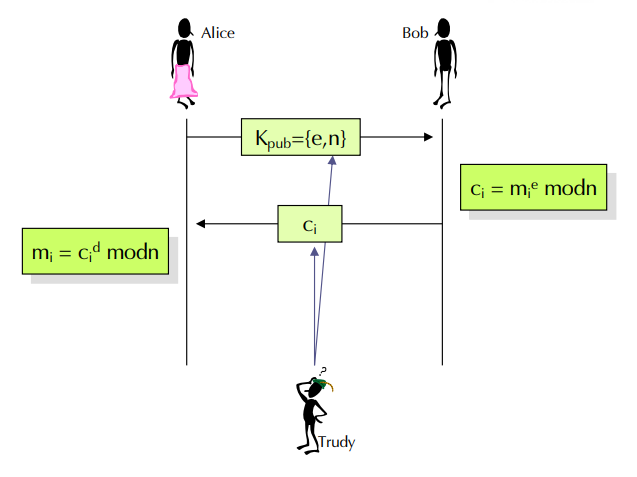
\includegraphics[width=0.8\textwidth]{RSAconf.png}
  \caption{Schema RSA per Confidenzialità}
  \label{fig:}
\end{figure}

\subsubsection{2. Firme Digitali}
Per firmare, Alice usa la sua \textbf{chiave privata} (per dimostrare di essere lei). Bob verifica la firma usando la \textbf{chiave pubblica} di Alice.
\begin{itemize}
    \item \textbf{Firma (Alice):} $f = m^d \mod n$ (dove $m$ è il messaggio o, più realisticamente, l'hash del messaggio).
    \item Alice invia a Bob la coppia $\{m, f\}$.
    \item \textbf{Verifica (Bob):} Bob calcola $m' = f^e \mod n$. Se $m' = m$, la firma è valida.
\end{itemize}
Questo garantisce non ripudio: solo Alice (che possiede $d$) può aver generato $f$.

\begin{figure}[H]
  \centering
  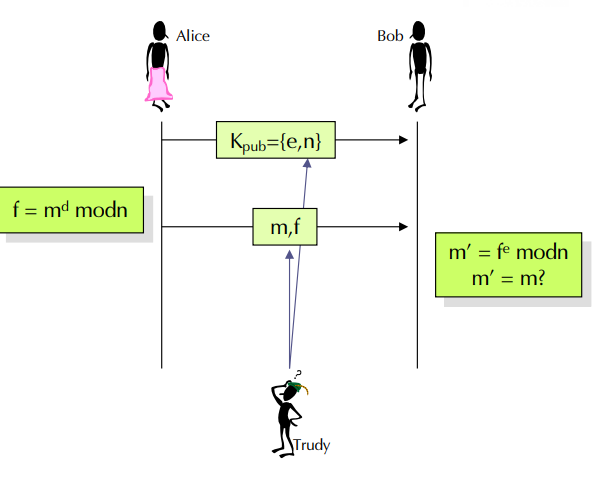
\includegraphics[width=0.8\textwidth]{RSAfirme.png}
  \caption{Schema RSA per Firme Digiali}
  \label{fig:}
\end{figure}
\subsubsection{3. Instaurazione di Chiavi Effimere}
Poiché RSA è computazionalmente lento, non si usa per cifrare messaggi lunghi. Si usa invece un approccio ibrido:
\begin{enumerate}
    \item Bob genera una chiave simmetrica $r$ (es. per DES o AES), detta chiave effimera o di sessione.
    \item Bob cifra $r$ usando la $K_{pub}$ di Alice (RSA): $c = r^e \mod n$.
    \item Bob invia $c$ ad Alice.
    \item Alice decifra $c$ con la sua $K_{priv}$ (RSA) e ottiene $r$: $r = c^d \mod n$.
    \item Ora Bob e Alice condividono la chiave simmetrica $r$ e la usano per cifrare il resto della comunicazione (es. $c_i = DES_r(m_i)$), che è molto più efficiente.
\end{enumerate}

\begin{figure}[H]
  \centering
  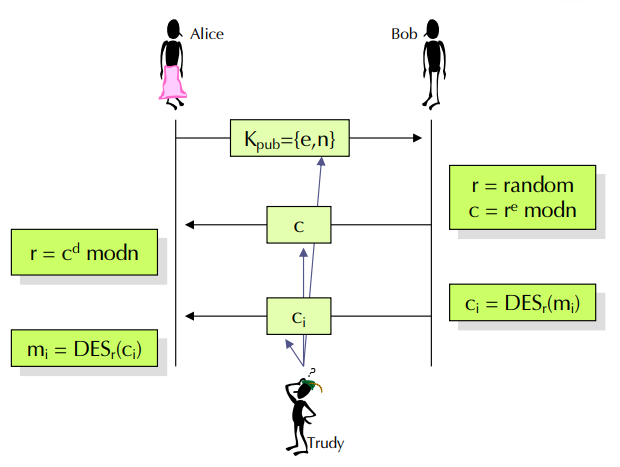
\includegraphics[width=0.8\textwidth]{RSAkey.png}
  \caption{Schema RSA per Scambio Chiavi}
  \label{fig:}
\end{figure}

\subsection{Sicurezza e Uso Pratico di RSA}
\begin{itemize}
    \item \textbf{Padding:} Non si deve mai usare RSA "puro" (textbook RSA). Se $m$ è piccolo (es. $m^e < n$), un attaccante può calcolare $m = \sqrt[e]{c}$. Per evitare questo e altri attacchi, si aggiunge un \textbf{padding} (riempimento, spesso casuale) al messaggio $m$ prima di cifrarlo. Gli standard PKCS (Public Key Cryptography Standard) definiscono come applicare correttamente il padding.
    \item \textbf{Lunghezza Chiave:} La sicurezza dipende dalla grandezza di $n$. Oggi, chiavi $n$ più corte di 1024 o 2048 bit non sono considerate sicure.
    \item \textbf{Efficienza:} La generazione delle chiavi è lenta. La cifratura (con $e$ piccolo) è veloce, la decifratura (con $d$ grande) è lenta.
\end{itemize}

\section{Protocollo Diffie-Hellman (DH)}
DH (1976) è stato il primo meccanismo asimmetrico pubblicato. Il suo unico obiettivo è lo \textbf{scambio sicuro di una chiave effimera} $K$.
Basa la sua sicurezza sulla difficoltà del \textbf{problema del logaritmo discreto}: è semplice calcolare $b = a^i \mod p$, ma è difficile calcolare $i$ (il logaritmo) conoscendo $a, b, p$.

\subsection{Meccanismo di Base}
\begin{enumerate}
    \item Alice e Bob si accordano pubblicamente su un numero primo $p$ e un generatore $g$ (di $Z_p^*$).
    \item \textbf{Alice (privato):} Sceglie un numero segreto $Sa$ (random, $1 \le Sa < p$).
    \item \textbf{Alice (pubblico):} Calcola $T_a = g^{Sa} \mod p$ e lo invia a Bob.
    \item \textbf{Bob (privato):} Sceglie un numero segreto $Sb$ (random, $1 \le Sb < p$).
    \item \textbf{Bob (pubblico):} Calcola $T_b = g^{Sb} \mod p$ e lo invia ad Alice.
    \item \textbf{Calcolo Chiave (Alice):} Alice calcola $K = (T_b)^{Sa} \mod p = (g^{Sb})^{Sa} \mod p = g^{Sb \cdot Sa} \mod p$.
    \item \textbf{Calcolo Chiave (Bob):} Bob calcola $K = (T_a)^{Sb} \mod p = (g^{Sa})^{Sb} \mod p = g^{Sa \cdot Sb} \mod p$.
\end{enumerate}
Alice e Bob hanno ottenuto la stessa chiave segreta $K$ senza mai trasmetterla. Un attaccante (Trudy) che osserva $p, g, T_a, T_b$ non può calcolare $K$ perché non conosce $Sa$ o $Sb$, e non può ricavarli a causa della difficoltà del logaritmo discreto.

\begin{figure}[H]
  \centering
  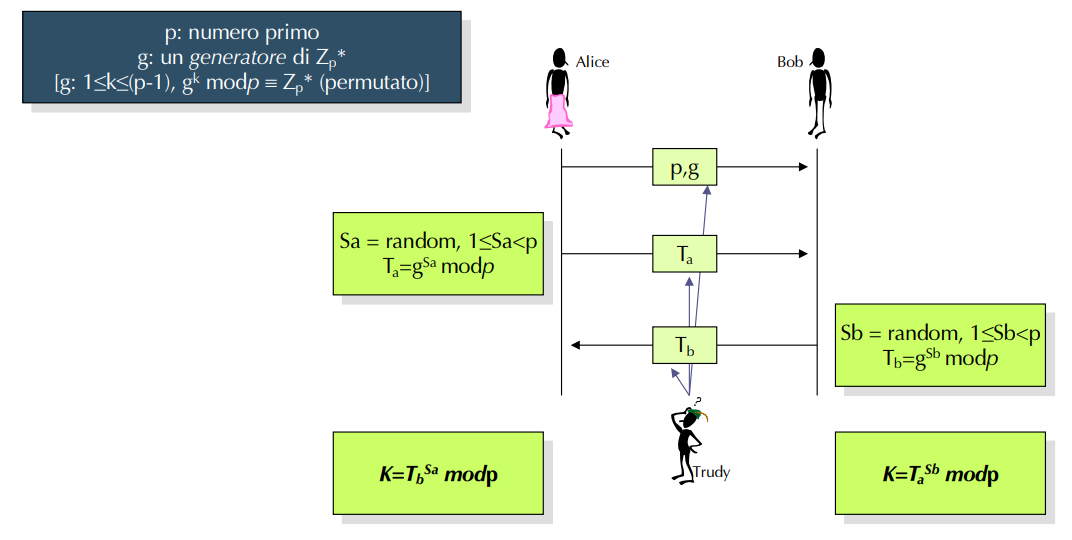
\includegraphics[width=0.8\textwidth]{DiffieHellman.png}
  \caption{Schema protocollo Diffie Hellman}
  \label{fig:}
\end{figure}
\subsection{Sicurezza di DH}
\begin{itemize}
    \item \textbf{Attacchi Passivi:} DH è sicuro contro l'intercettazione (come visto sopra).
    \item \textbf{Attacchi Attivi (Man-in-the-Middle):} DH è vulnerabile all'attacco "Man-in-the-Middle" (MitM) perché lo scambio non è autenticato. Trudy può fingersi Bob con Alice e Alice con Bob, negoziando due chiavi separate e inoltrando i messaggi. Per prevenire ciò, DH viene quasi sempre usato insieme a meccanismi di autenticazione (es. firme digitali).
\end{itemize}

\section{Elliptic Curve Cryptography (ECC)}
ECC è un'evoluzione degli algoritmi asimmetrici. Si basa su problemi matematici (legati alle curve ellittiche) che sono considerati (ad oggi) ancora più difficili da risolvere rispetto alla fattorizzazione (RSA) o al logaritmo discreto (DH).
Il vantaggio principale è che ECC può offrire lo \textbf{stesso grado di sicurezza di RSA con chiavi molto più piccole} (es. 1/10 della dimensione). Questo rende le operazioni molto più veloci ed efficienti, aspetto cruciale per server o dispositivi con poche risorse.

\section{Public Key Infrastructure (PKI)}
\subsection{Il Problema dell'Autenticità}
Come detto, la crittografia asimmetrica richiede che un utente (Bob) ottenga una copia autentica della chiave pubblica di un altro utente (Alice). Se non c'è garanzia di autenticità, Bob è vulnerabile a un attacco MitM.

La soluzione è introdurre una \textbf{Certification Authority (CA)}, ovvero una terza parte fidata.
L'idea è: "Se Bob si fida della CA, e la CA garantisce (firma) che una certa chiave pubblica appartiene ad Alice, allora Bob può fidarsi di quella chiave pubblica".

\subsection{Certificati Digitali (X.509)}
Una PKI è l'infrastruttura (protocolli, policy, CA) che gestisce questo processo. Lo strumento operativo è il \textbf{certificato digitale} (lo standard più diffuso è X.509).

Un certificato X.509 è un documento digitale che lega un'identità a una chiave pubblica. I suoi campi principali sono:
\begin{itemize}
    \item \textbf{Identità dell'Utente (Subject):} Chi possiede la chiave (es. CN=argo.ing.unibs.it).
    \item \textbf{Chiave Pubblica dell'Utente:} La chiave $K_{pubA}$ che si sta certificando.
    \item \textbf{Identità della CA (Issuer):} Chi ha emesso e firmato il certificato (es. CN=Test CA).
    \item \textbf{Validità:} Un periodo (data di inizio e fine) durante il quale il certificato è valido.
    \item \textbf{Firma della CA:} L'hash di tutti i campi precedenti, cifrato con la chiave \emph{privata} della CA ($K_{privCA}$).
\end{itemize}

\begin{figure}[H]
  \centering
  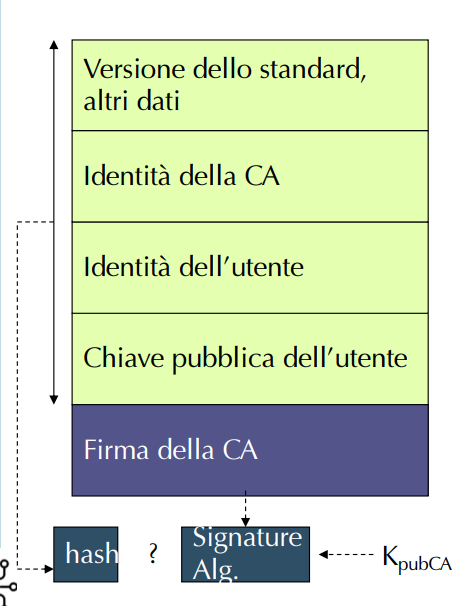
\includegraphics[width=0.8\textwidth]{X509.png}
  \caption{Schema campi certificato X.509}
  \label{fig:}
\end{figure}

\subsection{Processo di Verifica del Certificato}
\begin{enumerate}
    \item Alice invia a Bob il suo certificato, $CERT_A$ (firmato da $CA_{xz12a}$).
    \item Bob riceve $CERT_A$. Per fidarsi, deve verificare la firma.
    \item Bob estrae l'identità dell'Issuer ($CA_{xz12a}$).
    \item Bob cerca $CA_{xz12a}$ nella sua lista di \textbf{Root CA} attendibili (pre-installate nel suo OS o browser).
    \item Se la trova, estrae la $K_{pubCA}$ (che era nel certificato della CA stessa).
    \item Bob usa $K_{pubCA}$ per verificare la firma $S_{CA,xz12a}$ presente sul $CERT_A$ di Alice.
    \item Se la verifica ha successo, Bob sa che $CERT_A$ è autentico e integro. Ora può fidarsi della $K_{pubA}$ contenuta al suo interno per comunicare con Alice.
\end{enumerate}

\begin{figure}[H]
  \centering
  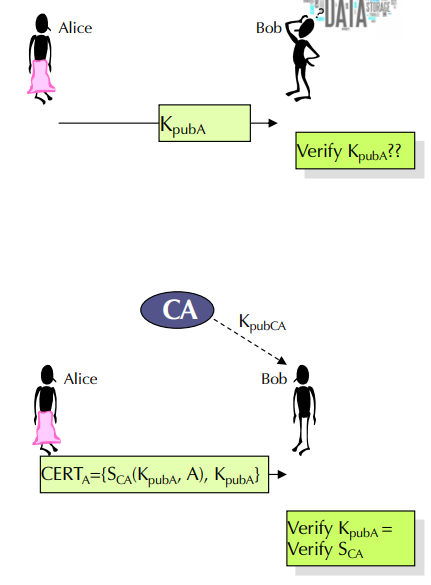
\includegraphics[width=0.8\textwidth]{cert.png}
  \caption{Schema verifica certficato}
  \label{fig:}
\end{figure}

\subsection{Catene di Certificati e Revoca}
\begin{itemize}
    \item \textbf{Root CA:} Le CA di cui ci si fida implicitamente (i loro certificati sono pre-installati) sono dette "Root CA". I loro certificati sono \emph{self-signed} (Issuer == Subject), poiché non c'è un'autorità superiore che li firmi.
    \item \textbf{Intermediate CA:} Per ragioni di sicurezza, le Root CA non firmano direttamente i certificati degli utenti finali. Firmano i certificati di "CA Intermedie" ($CA_1$), che a loro volta firmano i certificati degli utenti (Alice).
    \item \textbf{Catena (Chain of Trust):} Alice invia a Bob sia il suo certificato (firmato da $CA_1$) sia il certificato di $CA_1$ (firmato dalla $CA_{root}$). Bob verifica prima $CA_1$ usando la $CA_{root}$, e poi verifica Alice usando $CA_1$.
    \item \textbf{Revoca (CRL):} Se una chiave privata viene compromessa, il certificato corrispondente deve essere revocato prima della sua data di scadenza. Le CA pubblicano periodicamente una \textbf{Certificate Revocation List (CRL)}, una lista firmata dei numeri seriali dei certificati revocati. Prima di fidarsi di un certificato, Bob dovrebbe anche controllare che non sia presente nell'ultima CRL della CA.
\end{itemize} 
\end{document}

